\section{FSM utilizando ecuaciones \label{sec:s1}}



\begin{center}
	\begin{minipage}{10cm}
		Describir una FSM que resuelva el problema de detectar una secuencia de cuatro unos seguidos
		o cuatro ceros seguidos incluso secuencias traslapadas. Usar el estilo ``ONE - HOT'' utilizando 9 flip-flops para el estado.
		
		\enter
		
		Diseñar utilizando las ecuaciones de los flip-flops. Compilar y simular. Observar el resultado en el
		visor RTL.
	\end{minipage}
\end{center}


\enter

Como se usan ecuaciones, entonces se está describiendo detalladamente lo que hace 
la máquina en cada estado en el que se encuentra, por lo que se trata de una
descripcion por flujo de datos de bajo nivel.

\enter

\begin{figure}[ht]
	\centering
	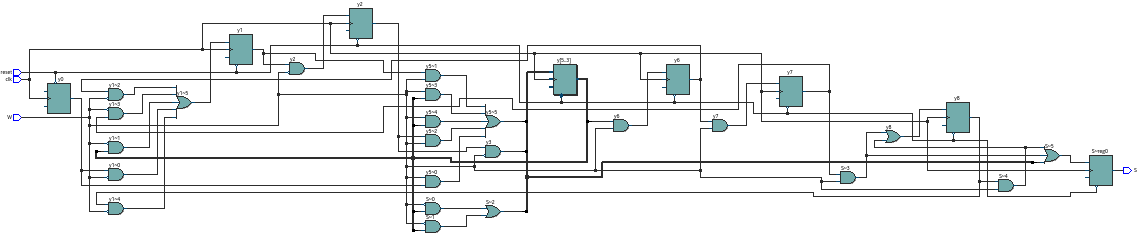
\includegraphics[scale=0.4]{fsm1hot_rtl.png}
	\caption{
		Diagrama RTL de la FSM, usando ecuaciones de la tabla \textit{One Hot}.
		\label{fig:fsm1hot_rtl}
	}
\end{figure}

\begin{figure}[ht]
	\centering
	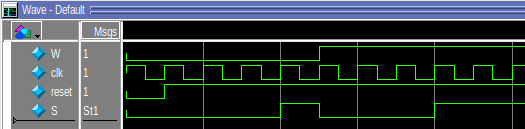
\includegraphics[scale=0.5]{fsm1hot_sim.png}
	\caption{
		Simulación de la FSM, usando ecuaciones de la tabla \textit{One Hot}.
		\label{fig:fsm1hot_sim}
	}
\end{figure}








\newpage
\begin{center}
	\begin{minipage}{10cm}
		Considerar la tabla ``ONE - HOT'' modificada.
		
		\enter
		
		Diseñar utilizando las ecuaciones de los flip-flops. Compilar y simular. Observar el resultado en el
		visor RTL.
	\end{minipage}
\end{center}

\enter


\begin{figure}[ht]
	\centering
	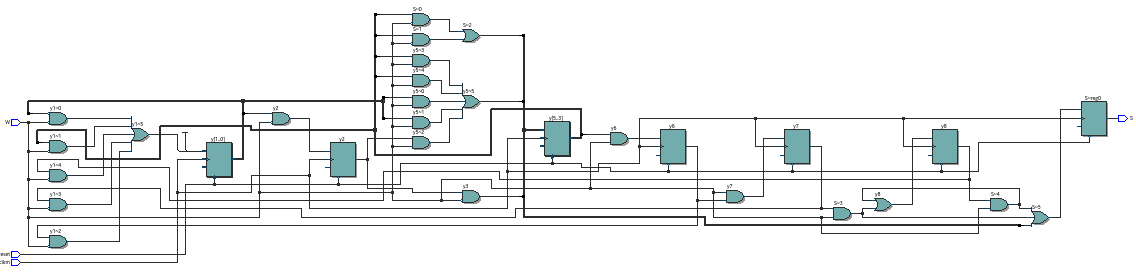
\includegraphics[scale=0.4]{fsm1hotmod_rtl.png}
	\caption{
		Diagrama RTL de la FSM, usando ecuaciones de la tabla \textit{One Hot} modificada.
		\label{fig:fsm1hotmod_rtl}
	}
\end{figure}

Se obtiene la misma simulación mostrada en la \autoref{fig:fsm1hot_sim}.

\enter

Observando los diagramas RTL, mostrados en la \autoref{fig:fsm1hot_rtl} y
\autoref{fig:fsm1hotmod_rtl}, la diferencia está en que la tabla \textit{one hot} modificada ahorra flip-flops al momento de implementar, además en la entrada se colocan compuertas lógicas en lugar del primer flip-flop que está en la descripción con tabla \textit{one hot}.

